%!TEX root = ../../thesis.tex

\section{Models}
\label{sec:coqa-models}

Given a passage $p$, the conversation history \{$q_1, a_1, \ldots q_{i-1}, a_{i-1}$\} and a question $q_i$, the task is to predict the answer ${a_i}$. Our task can be modeled as either a conversational response generation problem or a reading comprehension problem. We evaluate strong baselines from each class of models and a combination of the two on \sys{CoQA}.

\subsection{Conversational Models}

\begin{figure}[!t]
\begin{center}
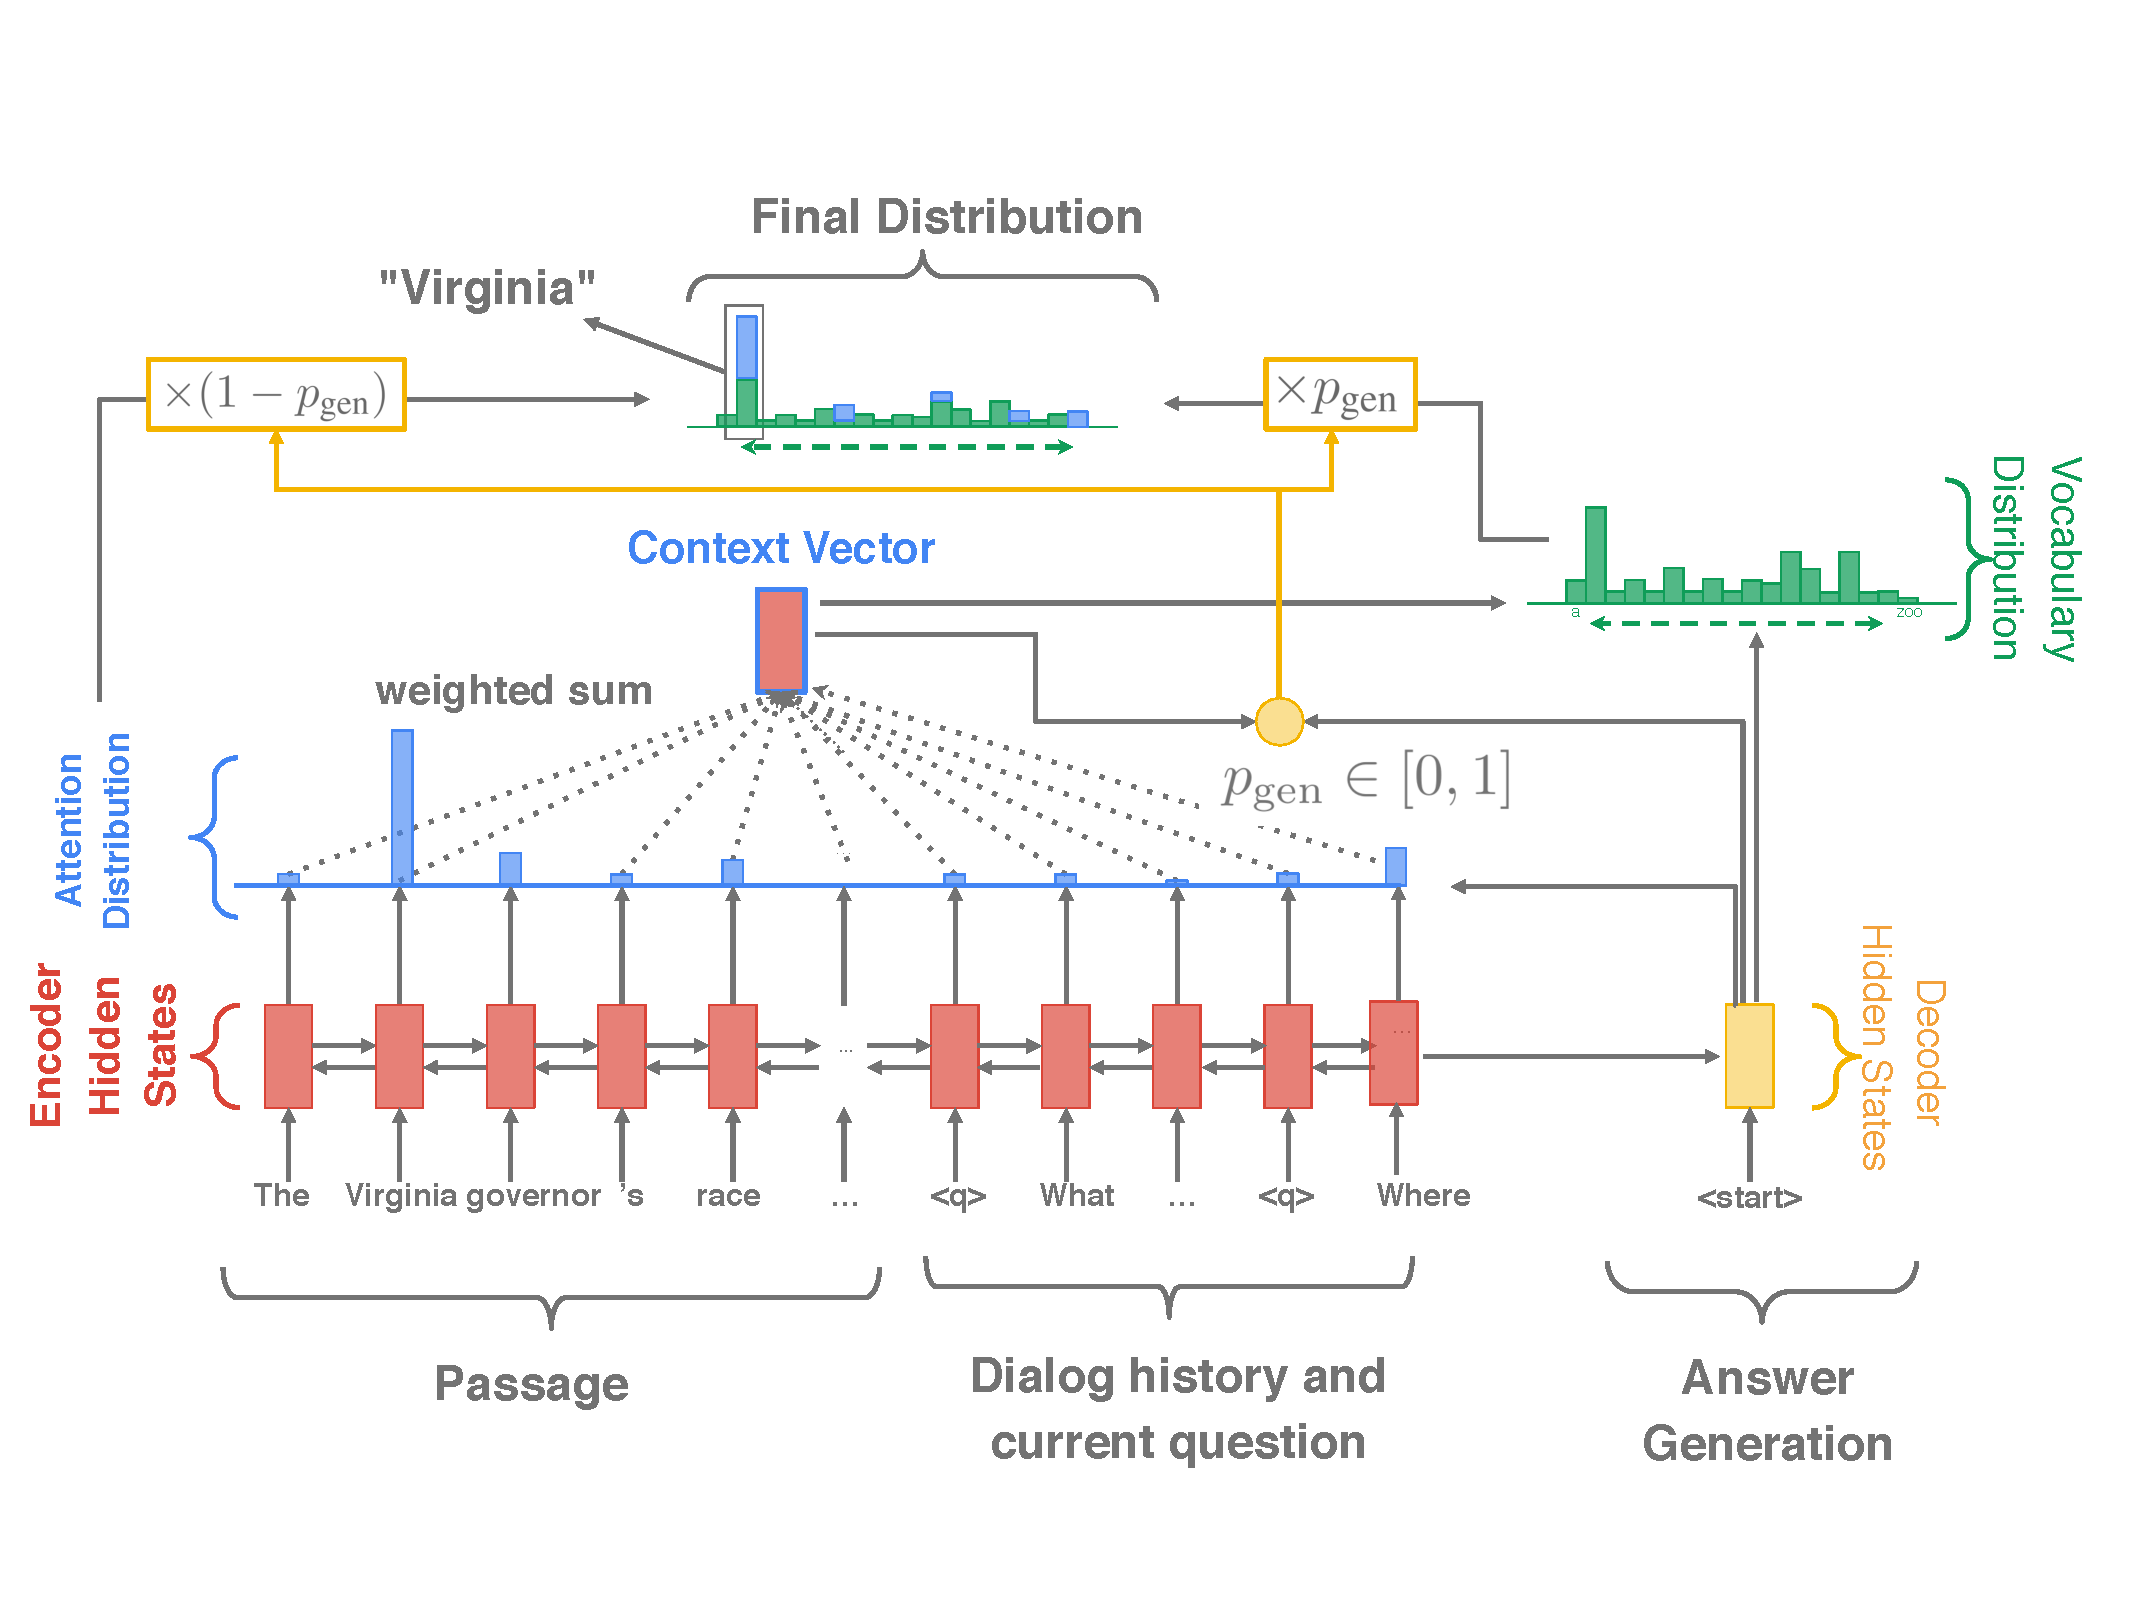
\includegraphics[height=9.5cm]{img/coqa_pgnet.pdf}
\end{center}
\longcaption{The pointer-generator network used for conversational question answering}{\label{fig:coqa-pgnet} The pointer-generator network used for conversational question answering. The figure is adapted from \newcite{see2017get}.}
\end{figure}

The basic goal of conversational models is to predict the next utterance based on its conversation history. Sequence-to-sequence (seq2seq) models~\cite{sutskever2014sequence} have shown promising results for generating conversational responses \cite{vinyals2015neural,li2016diversity,zhang2018personalizing}. Motivated by their success, we use a standard sequence-to-sequence model with an attention mechanism for generating answers. We append the passage, the conversation history (the question/answer pairs in the last $n$ turns) and the current question as, $p\; \mathrm{<}q\mathrm{>}\; q_{i-n} \;\mathrm{<}a\mathrm{>}\; a_{i-n}\; \ldots$ $\mathrm{<}q\mathrm{>}\; q_{i-1} \;\mathrm{<}a\mathrm{>}\; a_{i-1}\;$  $\mathrm{<}q\mathrm{>}\;q_i$, and feed it into a bidirectional LSTM encoder, where $\mathrm{<}q\mathrm{>}$ and $\mathrm{<}a\mathrm{>}$ are special tokens used as delimiters. We then generate the answer using a LSTM decoder which attends to the encoder states.

Moreover, as the answer words are likely to appear in the original passage, we adopt a copy mechanism in the decoder proposed for summarization tasks \cite{gu2016incorporating,see2017get}, which allows to (optionally) copy a word from the passage and the conversation history. We call this model the Pointer-Generator network~\cite{see2017get}, \sys{PGNet}. Figure~\ref{fig:coqa-pgnet} illustrates a full model of \sys{PGNet}. Formally, we denote the encoder hidden vectors by $\{\tilde{\mf{h}}_i\}$, the decoder state at timestep $t$ by $\mf{h}_t$ and the input vector by $\mf{x}_t$, an attention function is computed based on $\{\tilde{\mf{h}}_i\}$ and $\mf{h}_t$  as $\alpha_i$ (Equation~\ref{eq:attention}) and the context vector is computed as $\mf{c} = \sum_{i}{\alpha_i \tilde{\mf{h}}_i}$ (Equation~\ref{eq:context-vector}).

For a copy mechanism, it first computes the \ti{generation probability} $p_{\text{gen}} \in [0, 1]$ which controls the probability that it generates a word from the full vocabulary $\mathcal{V}$ (rather than copying a word) as:

\begin{equation}
    p_{\text{gen}} = \sigma\left({\mf{w}^{(c)}}^{\intercal}\mf{c} + {\mf{w}^{(x)}}^{\intercal}\mf{x}_t + {\mf{w}^{(h)}}^{\intercal}\mf{h}_t + b\right).
\end{equation}

The final probability distribution of generating word $w$ is computed as:
\begin{equation}
    P(w) = p_{\text{gen}}P_{\text{vocab}}(w) + (1 - p_{\text{gen}})\sum_{i: w_i = w}\alpha_i,
\end{equation}
where $P_{\text{vocab}}(w)$ is the original probability distribution (computed based on $\mf{c}$ and $\mf{h}_t$) and $\{w_i\}$ refers to all the words in the passage and the dialogue history. For more details, we refer readers to \cite{see2017get}.


\subsection{Reading Comprehension Models}
The second class of models we evaluate is the neural reading comprehension models. In particular, the models for the span prediction problems can't be applied directly, as a large portion of the \sys{CoQA} questions don't have a single span in the passage as their answer, e.g., $Q_3$, $Q_4$ and $Q_5$ in Figure~\ref{fig:coqa-example}. Therefore, we modified the \sys{Stanford Attentive Reader} model we described in Section~\ref{sec:sar} for this problem. Since the model requires text spans as answers during training, we select the span which has the highest lexical overlap (F1 score) with the original answer as the gold answer. If the answer appears multiple times in the story we use the rationale to find the correct one. If any answer word does not appear in the passage, we fall back to an additional \textit{unknown} token as the answer (about 17\%). We prepend each question with its past questions and answers to account for conversation history, similar to the conversational models.

\subsection{A Hybrid Model}
The last model we build is a \ti{hybrid} model, which combines the advantages of the aforementioned two models. The reading comprehension models can predict a text span as an answer, while they can't produce answers that do not overlap with the passage. Therefore,  we combine \sys{Stanford Attentive Reader} with \sys{PGNet} to address this problem since \sys{PGNet} can generate free-form answers effectively. In this hybrid model, we use the reading comprehension model to first point to the answer evidence in text, and \sys{PGNet} naturalizes the evidence into the final answer. For example, for Q$_5$ in Figure~\ref{fig:coqa-example}, we expect that the reading comprehension model first predicts the rationale R$_5$ \ti{Her granddaughter Annie was coming over in the afternoon and Jessica was very excited to see her. Her daughter Melanie and Melanie’s husband Josh were coming as well.}, and then \sys{PGNet} generates A$_5$ \ti{Annie, Melanie and Josh} from R$_5$.

We make a few changes to both models based on empirical performance. For the \sys{Stanford Attentive Reader} model, we only use rationales as answers for the questions with an non-extractive answer. For \sys{PGNet}, we only provide current question and span predictions from the the \sys{Stanford Attentive Reader} model as input to the encoder. During training, we feed the oracle spans into \sys{PGNet}.
